\hypertarget{section-introduction-and-goals}{%
\section{Introduction and Goals}\label{section-introduction-and-goals}}

Describes the relevant requirements and the driving forces that software
architects and development team must consider. These include

\begin{itemize}
\item
  underlying business goals,
\item
  essential features,
\item
  essential functional requirements,
\item
  quality goals for the architecture and
\item
  relevant stakeholders and their expectations
\end{itemize}

\hypertarget{_requirements_overview}{%
\subsection{Requirements Overview}\label{_requirements_overview}}

\textbf{Contents}

Short description of the functional requirements, driving forces,
extract (or abstract) of requirements. Link to (hopefully existing)
requirements documents (with version number and information where to
find it).

\textbf{Motivation}

From the point of view of the end users a system is created or modified
to improve support of a business activity and/or improve the quality.

\textbf{Form}

Short textual description, probably in tabular use-case format. If
requirements documents exist this overview should refer to these
documents.

Keep these excerpts as short as possible. Balance readability of this
document with potential redundancy w.r.t to requirements documents.

See \href{https://docs.arc42.org/section-1/}{Introduction and Goals} in
the arc42 documentation.

\hypertarget{_quality_goals}{%
\subsection{Quality Goals}\label{_quality_goals}}

\textbf{Contents}

The top three (max five) quality goals for the architecture whose
fulfillment is of highest importance to the major stakeholders. We
really mean quality goals for the architecture. Don't confuse them with
project goals. They are not necessarily identical.

Consider this overview of potential topics (based upon the ISO 25010
standard):

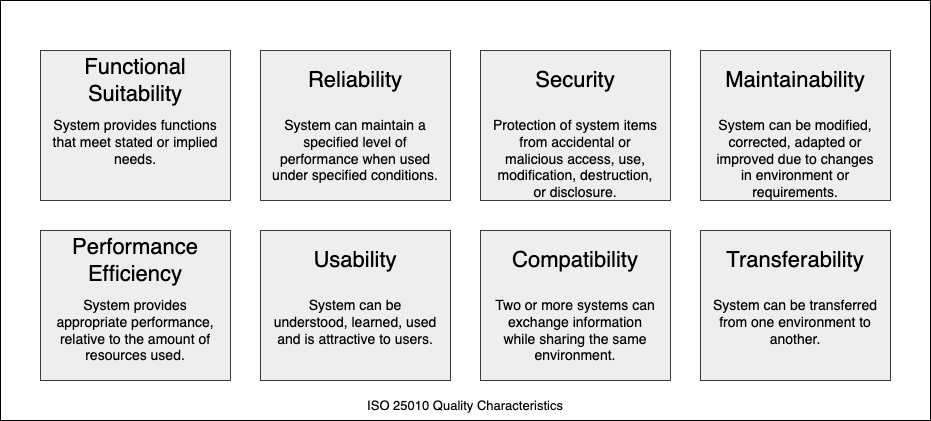
\includegraphics{../images/01_2_iso-25010-topics-EN.drawio.png}

\textbf{Motivation}

You should know the quality goals of your most important stakeholders,
since they will influence fundamental architectural decisions. Make sure
to be very concrete about these qualities, avoid buzzwords. If you as an
architect do not know how the quality of your work will be
judged\ldots{}

\textbf{Form}

A table with quality goals and concrete scenarios, ordered by priorities

\hypertarget{_stakeholders}{%
\subsection{Stakeholders}\label{_stakeholders}}

\textbf{Contents}

Explicit overview of stakeholders of the system, i.e. all person, roles
or organizations that

\begin{itemize}
\item
  should know the architecture
\item
  have to be convinced of the architecture
\item
  have to work with the architecture or with code
\item
  need the documentation of the architecture for their work
\item
  have to come up with decisions about the system or its development
\end{itemize}

\textbf{Motivation}

You should know all parties involved in development of the system or
affected by the system. Otherwise, you may get nasty surprises later in
the development process. These stakeholders determine the extent and the
level of detail of your work and its results.

\textbf{Form}

Table with role names, person names, and their expectations with respect
to the architecture and its documentation.

\begin{longtable}[]{@{}
  >{\raggedright\arraybackslash}p{(\columnwidth - 4\tabcolsep) * \real{0.2000}}
  >{\raggedright\arraybackslash}p{(\columnwidth - 4\tabcolsep) * \real{0.4000}}
  >{\raggedright\arraybackslash}p{(\columnwidth - 4\tabcolsep) * \real{0.4000}}@{}}
\toprule
\begin{minipage}[b]{\linewidth}\raggedright
Role/Name
\end{minipage} & \begin{minipage}[b]{\linewidth}\raggedright
Contact
\end{minipage} & \begin{minipage}[b]{\linewidth}\raggedright
Expectations
\end{minipage} \\
\midrule
\endhead
\emph{\textless Role-1\textgreater{}} &
\emph{\textless Contact-1\textgreater{}} &
\emph{\textless Expectation-1\textgreater{}} \\
\emph{\textless Role-2\textgreater{}} &
\emph{\textless Contact-2\textgreater{}} &
\emph{\textless Expectation-2\textgreater{}} \\
\bottomrule
\end{longtable}
